\documentclass{article}
% Milestone snapshot: November 7, 2026.
% Numeric evidence (paths relative to the repository):
% runs/grasp_7to10/{results,audit_policy}.json and original contact traces
% doc/cleanup/2026-11-07/historical_results.json
% data/interaction_pose_v2_5000_20261107/status.json
% data/interaction_pose_v2_early_quality_20261107/status.json
% doc/cleanup/2026-11-07/baseline_pilot_10/ and pose_training_smoke/
% Preserve metric versions when adding future learned-pose results.
\usepackage{xcolor}
\usepackage[preprint]{corl_2024}
\usepackage{amsmath,amssymb,booktabs,graphicx,tikz}
\usetikzlibrary{arrows.meta,positioning}

\title{From Part Prompts to Interaction Poses:\\Toward Stable Grasping in Door Opening}
\author{Jinyoon Kim\\University of Virginia\\Interactive Robotics Course Project}
\hypersetup{pdftitle={From Part Prompts to Interaction Poses: Toward Stable Grasping in Door Opening},
  pdfauthor={Jinyoon Kim},pdfsubject={Project milestone report}}

\begin{document}
\maketitle

\begin{abstract}
Successful door motion does not guarantee a stable handle grasp. In our
ten-start development pilot, pretrained MolmoBot opened nine doors, but only
two runs satisfied the grasp-retention criterion. Our goal is to improve
opening with a stable grasp over this baseline. Because MolmoBot already
receives a target-part point prompt, we propose converting part information
into an explicit interaction pose with a defined role in execution. Currently,
we supply privileged oracle poses to test the value of accurate grasp targets.
The final method will predict TCP position, orientation and gripper
configuration from images, robot state and the existing point prompt, a part
mask, or both. A point-conditioned pose-head prototype is implemented and passes
a small Train-only integration test; full training, mask conditioning and the
final Test comparison remain planned.
\end{abstract}
\keywords{Part-aware manipulation, grasp stability, interaction poses}

\section{Introduction}
\label{sec:intro}
Our objective is to improve stable handle grasping during door opening over
pretrained MolmoBot. The local baseline gap between ordinary opening and
grasp-retention success motivates establishing a suitable handle grasp and
retaining it while opening. These pilot observations are not benchmark-wide
estimates, and failing the criterion does not prove physical grasp loss in
every case.

We initially considered supplying handle masks to MolmoBot in
MolmoSpaces~\citep{kim2026molmospaces,deshpande2026molmobot}. However, the native
door-opening configuration already supplies a target-part image point with an
initial conditioning image. A mask may add shape and extent, but its incremental
value must be tested. Existing localization does not fully specify gripper
orientation, closure or a pose suited to maintaining contact as the door moves.

We propose a supervised tool-center-point (TCP) pose and gripper configuration
that a local execution mechanism explicitly consumes. This gives part inputs
a measurable control role; supplying a point or mask alone does not establish
effective use. The work has two stages. First, our current oracle study supplies
expert-derived poses to test whether accurate targets help. Second, an implemented
pose-head prototype will be trained to predict those targets from part information
and current observations, then use the same execution mechanism. The final goal is improved stable-grasp
opening over the baseline while preserving ordinary opening success.

\section{Related Work}
\label{sec:related}
\textbf{Simulation and pretrained policies.}
MolmoSpaces provides indoor simulation assets, data-generation tools and
benchmarking infrastructure~\citep{kim2026molmospaces}. MolmoBot learns
manipulation from large-scale synthetic demonstrations and supports optional
image-point conditioning~\citep{deshpande2026molmobot}. We use the released
RB-Y1 multitask policy and MuJoCo environment, adding grasp-stage guidance
rather than training a complete policy from scratch.

\textbf{From local affordances to geometric actions.}
Where2Act connects articulated-part actionability to contact-conditioned
interaction parameters, including gripper orientation~\citep{mo2021where2act}.
PerAct predicts structured 6-DoF manipulation actions from language and
RGB-D observations~\citep{shridhar2023peract}; Act3D predicts end-effector
keyposes using a spatial feature representation~\citep{gervet2023act3d}.
These works motivate representing how to interact, in addition to where.
Our approach preserves MolmoBot for full-task behavior and studies whether
part-conditioned pose guidance improves stable grasping during door opening.

\section{Problem Definition}
\label{sec:problem}
At time $t$, the native policy observes camera images $I_t$, robot state $s_t$,
task instruction $\ell$, and native target-point/conditioning-image input $p$.
It produces a chunk of joint-space actions. The proposed pose module additionally
uses part evidence $z_t$: the existing point prompt, a part mask, or both.
The final learned mapping is $\hat y_t=f_\theta(I_t,s_t,\ell,z_t)$, with
$\hat y_t=(\hat T^{B_t}_{G},\hat c)$, where
$\hat T^{B_t}_{G}\in SE(3)$ is a desired TCP pose in the current robot-base
frame and $\hat c$ specifies gripper configuration. The reported control pilots
use supplied oracle targets. The new predictor has undergone only a four-update
integration test, rather than the planned full training run.

\textbf{Data.} We prepared 5,004 pose references from official Train
demonstrations across 977 contributing houses. The early-grasp view retains 4,866 targets
and 19,464 observation--target pairs. We use official Train for learning and
official Val as Test, with 187 currently available early-grasp targets.
Selection requires source grasp flags and measured closure before 10\% opening,
with no prior major opening. Four preceding observations share each target in
their respective robot-base frames. These are recorded expert TCP references;
full-task grasp retention is not certified by the source labels.

\textbf{Objective and evaluation.} Let $S_{\rm open}$ denote reaching the
configured opening fraction of 0.67 and $S_{\rm grasp}$ denote acquiring a
qualifying grasp before substantial opening and retaining it through completion.
We aim to increase $J_{\rm stable}(\pi)=\Pr_\pi(S_{\rm open}\land S_{\rm grasp})$
over frozen MolmoBot, also reporting ordinary opening, grasp acquisition and
pose error. Retention diagnostics sample forces and handle-relative TCP motion
at 10\,Hz; 2\,cm/10-degree limits are proxies under validation. Comparisons
share starts, seeds and action budgets, disclosing additional sensing.
We separate Train/Test houses; Test never selects settings or checkpoints, and
prior inspections are recorded. The existing 197 expert trajectories form the
Test base. Verification and expansion toward 400 total cases are deferred;
candidate identities do not establish qualification. This split does not prove
absence from MolmoBot pretraining.

\section{Technical Approach}
\label{sec:method}
\textbf{Stage 1: supplied oracle poses.} In the full-start policy pilot, we supply an expert-derived
grasp pose and apply bounded corrections around handle contact. This tests
whether a more specific target helps beyond a grasp guard alone, before
training a predictor. MolmoBot still generates approach and opening actions;
expert action sequences are not replayed in this comparison.

\textbf{Stage 2: implemented pose-head prototype.} A frozen DINOv2 encoder
extracts global and point-local features from three current RGB views. A
three-layer transformer combines them with robot joints and push/pull context,
predicting TCP translation, rotation, active arm and finger-displacement span.
Only the added head is trained. Current-frame simulator handle points are an
additional input beyond MolmoBot's initial-image prompt; this distinction must
be controlled in comparisons. Missing points have explicit visibility flags.
Masks remain a future input extension. Expert poses and arm labels supervise
training but are not inference inputs.

\begin{figure}[!ht]
\centering
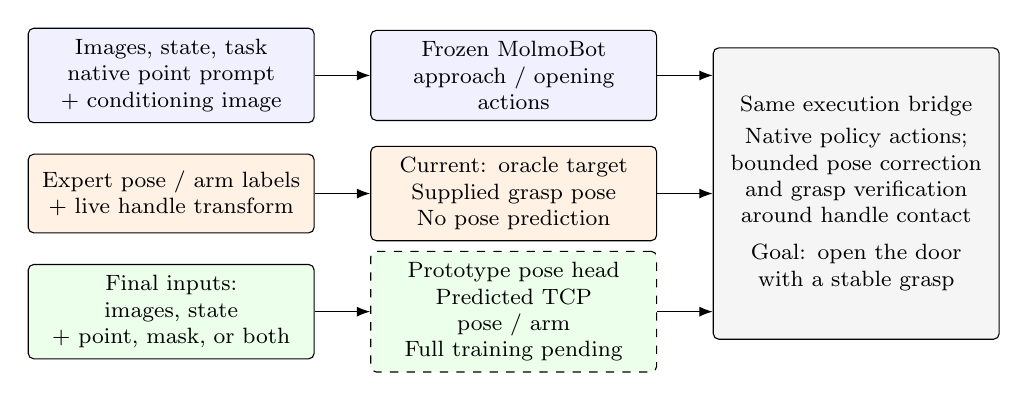
\begin{tikzpicture}[>=Latex,font=\footnotesize,
  box/.style={draw,rounded corners=2pt,align=center,text width=3.35cm,
              minimum height=1.0cm,inner sep=4pt}]
  \node[box,fill=blue!6] (native) at (0,0) {Images, state, task\\native point prompt\\+ conditioning image};
  \node[box,fill=blue!6] (policy) at (4.35,0) {Frozen MolmoBot\\approach / opening\\actions};
  \node[box,fill=orange!10] (expert) at (0,-1.5) {Expert pose / arm labels\\+ live handle transform};
  \node[box,fill=orange!10] (oracle) at (4.35,-1.5) {Current: oracle target\\Supplied grasp pose\\No pose prediction};
  \node[box,fill=green!8] (part) at (0,-3) {Final inputs: images, state\\+ point, mask, or both};
  \node[box,fill=green!8,dashed] (pose) at (4.35,-3) {Prototype pose head\\Predicted TCP pose / arm\\Full training pending};
  \node[box,fill=gray!8,minimum height=3.7cm] (control) at (8.7,-1.5) {Same execution bridge\\[2pt]Native policy actions;\\bounded pose correction\\and grasp verification\\around handle contact\\[4pt]Goal: open the door\\with a stable grasp};
  \draw[->] (native)--(policy);
  \draw[->] (part)--(pose);
  \draw[->] (expert)--(oracle);
  \draw[->] (policy.east)--(control.west |- policy.east);
  \draw[->] (oracle.east)--(control.west);
  \draw[->] (pose.east)--(control.west |- pose.east);
\end{tikzpicture}
\caption{Oracle targets (orange) and the pose-head prototype (green) feed the
same execution bridge. Full training and mask inputs remain planned.}
\label{fig:method}
\end{figure}

\textbf{Supervised pose target.} For a recorded grasp pose $T^{W}_{G^*}$,
the target at an earlier observation is
$T^{B_t}_{G^*}=(T^{W}_{B_t})^{-1}T^{W}_{G^*}$.
The prototype uses Smooth L1 for translation and finger span, squared rotation
matrix distance, and cross-entropy for arm selection. Finger span is a measured
displacement proxy; native execution still uses guarded open/close commands.

\textbf{Execution mechanism.} The bridge converts bounded local corrections
into native relative commands, verifies contact and refreshes policy actions
after intervention. Oracle targets use expert handle-relative poses and live
handle transforms. Initial alignment alone does not ensure retention; opening
also requires feedback.

\textbf{Controls and training plan.} Compare frozen MolmoBot, a grasp guard,
oracle correction and learned pose guidance. Point/mask ablations will test
input dependence. Full training is pending: 20,000 optimizer updates, effective
batch four and Train diagnostics every 500 updates. The final checkpoint is
fixed before Test evaluation.

\section{Preliminary Results}
\label{sec:results}
\textbf{Local grasp acquisition: 7/10 to 10/10.} We first isolated grasping by
replaying the expert approach, then executing a local controller with an
expert-derived TCP target. On the same ten Train development cases, a wider
closing-position tolerance (20\,mm rather than 12\,mm) and bounded base recovery
improved sustained bilateral contact from 7/10 to 10/10 (Table~\ref{tab:contact}).
Each controller had 120 decisions (12 seconds), with privileged expert targets
and simulator handle/contact state. This measures local acquisition after an
expert approach, not full-start opening or force-qualified opening retention.

\begin{table}[!ht]
\centering
\caption{Retained local grasp comparison after expert approach. Success requires
bilateral finger contact throughout the final second of the 120-decision test.}
\label{tab:contact}
\begin{tabular}{lc}
\toprule
Controller & Sustained local contact\\
\midrule
Original 12\,mm closing gate & 7/10\\
20\,mm closing gate + bounded base recovery & 10/10\\
\bottomrule
\end{tabular}
\end{table}

Three workers finished simulation but failed a $10^{-8}$\,m reference check.
Post-hoc review confirmed identical discrete outcomes and trajectory differences
below 0.1\,mm/0.05 degrees. Original error statuses and success labels are preserved.

\textbf{Full-start MolmoBot comparison.} In a separate ten-start Train pilot,
MolmoBot generates approach and opening actions from the original closed-door
states. Table~\ref{tab:oracle} shows the baseline gap: 9/10 ordinary openings
versus 2/10 retained-grasp openings, our primary improvement target.

\begin{table}[!ht]
\centering
\caption{Completed ten-start Train development pilot, seed 42, 400-action budget.
Retained-grasp values use the historical pilot criterion.}
\label{tab:oracle}
\begin{tabular}{lcc}
\toprule
Method & Opening threshold & Retained-grasp opening\\
\midrule
Frozen MolmoBot & 9/10 & 2/10\\
MolmoBot + grasp guard & 10/10 & 3/10\\
Guard + oracle pose correction & 8/10 & 4/10\\
\bottomrule
\end{tabular}
\end{table}

All 30 rollouts matched initial inputs and first policy proposals. Retained-grasp
opening rises from 2/10 to 3/10 with the guard and 4/10 with oracle correction,
but oracle ordinary opening falls to 8/10. This tradeoff does not establish
overall improvement or learned-model performance.

\begin{samepage}
\textbf{Data and training readiness.} The source data and early-grasp indices
are prepared. The new pipeline extracted real DINOv2 features from four Train observations of one
trajectory, completed four optimizer updates, saved and reloaded a checkpoint,
and produced an offline Train pose-error report without accessing Test.
This verifies implementation, not learned grasping performance. No full
20,000-update training or learned-policy GPU evaluation has been run.\par
\end{samepage}

\textbf{Supporting diagnostics.} Fractional mask support preserved all 21
visible handles in saved preprocessing checks; a 50\%-foreground patch rule
erased 15. Three expert command replays opened 3/3 doors in each of two noise
modes, but a newer onset-based retention metric passed only 1/3 and 0/3.
Those rates use different semantics from Table~\ref{tab:oracle}; a declared
ten-step continuation was added after source-recorded success to observe
holding. These checks motivate further metric and controller-compatibility
review rather than certifying the entire Test set.

Next, we will train for 20,000 updates and compare predicted poses with frozen
MolmoBot on matched starts. Test verification/expansion toward 400 cases is
deferred; action-candidate scoring remains a separate optional direction.

% Keep the report and references within four pages; the GenAI appendix is separate.
\bibliography{references}

\clearpage
\appendix
\section{GenAI Use}
Generative AI (OpenAI Codex) helped me analyze the dataset, inspect robot
motions, and identify failure cases and possible causes. When I asked about
research concepts relevant to this project, it suggested related papers for me
to explore. It also helped refine the organization, clarity and wording of
this report.

\end{document}
